\documentclass{article}
\usepackage[utf8]{inputenc}
\usepackage{amsmath}
\usepackage{xcolor}
\usepackage{hyperref}
\usepackage{graphicx}

\title{IN3160: Oblig3}
\author{Trym Auren}
\date{Februar 2023}

\begin{document}

    \maketitle
    \tableofcontents
    \section*{a}
        \addcontentsline{toc}{section}{a}
        The output data signal changes at 450ns.
        During run:
        - \texttt{mclk} (clock) switch between low and high. One clock cycle lasts for 100 ns.
        \begin{enumerate}
            \item At start of run: \texttt{$rst_n$} (reset) is '0', switches to '1' after 100 ns.\\
                Elapsed time: 100 ns.
            \item Clock has gone through 1 cycle during this time. Since reset has been '0' throughout, \texttt{data(1,2,3,4,5)} has been assigned the value '0'.\\
                Elapsed time: 100 ns. 
            \item When reset is now set to high (1) after 100 ns, the if- test \texttt{elsif rising-edge} is executed two times (because of two elapsed clock- cycles), but \texttt{data(1,2,3,4,5)} is still '0', because \texttt{indata} is '0'.\\
                Elapsed time: 200 ns. 
            \item Now \texttt{indata} is assigned "11110000". Since reset is '1', \texttt{data1} is set to \texttt{indata = "11110000"} when the bulletpoint above (the previous process) is finished.\\
                Elapsed time: 200 ns.
            \item This time, \texttt{data2} is set to \texttt{data1} immediately, since its a variable. At the end of the process, \texttt{data3} is set to \texttt{data2}.\\
                Elapsed time: 300 ns.
            \item This time, \texttt{data4} is set to \texttt{data3} immediately, since its a variable. At the end of the process, \texttt{data5} is set to \texttt{data4}.\\
                Elapsed time: 400 ns.
            \item When the next process is done (this is normally done after 50 ns + minor delay), \texttt{data5} is finally the same value as \texttt{"11110000"}, and outdata is set to this value. This happens at 450 ns.\\
                Elapsed time: 500 ns.
        \end{enumerate}
        \begin{description}
            \item Note: Elapsed time: xx ns does not mean elapsed time right after previous described action, but is more of an index. 
        \end{description}

    \section*{b}
        \addcontentsline{toc}{section}{b}
        The output data signal changes at 750 ns. \\
        The output data signal is equal to "UUUUUUUU" at 50 ns, because the signal is not set before 100 ns.

    \section*{c}
        \addcontentsline{toc}{section}{c}
        \texttt{output(7 downto 6)} is always equal to \texttt{output(3 downto 2)}, because both standard logic vectors are set to the same signal, and the value of the signal assigned to \texttt{output(7 downto 6)} is not changed before after the process is done with an iteration. \\
        \texttt{output(5 downto 4)} is always different from \texttt{output(1 downto 0)}, because the vectors are assigned a variable, which is updated between the update of \texttt{output(1 downto 0)} and \texttt{output(5 downto 4)}. \\
        I.e., the difference lies in changing value of variables, which happens when the process is running, versus changing value of signals. 

    \section*{d}
        \addcontentsline{toc}{section}{d}
        The question boils down to what a sensitivity list is, and how the process is dependent on the list. When \texttt{sig1} and \texttt{sig2} is removed from the sensitivity list, the process is only invoked when there is a change in \texttt{indata} - the last parameter remaining. Since nothing changes to \texttt{indata} before after 100 ns (and then after 200 ns), the process will not run until at 100 ns (and at 200 ns). At task \textbf{c}, the process is triggered immediately at startup, because it listens to \texttt{sig1} and \texttt{sig2}.

    \section*{Figures}
        \addcontentsline{toc}{section}{Figures}
        \begin{figure}[!ht]
            \centering
            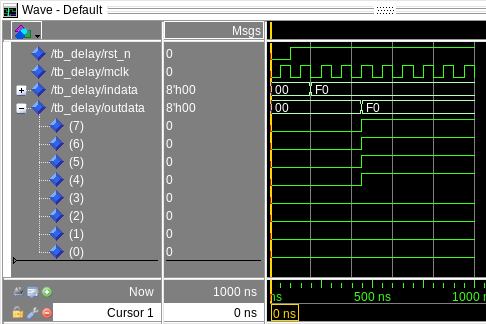
\includegraphics[width = \textwidth]{figur1.png}
            \caption{Task a}
            \label{fig:figure1}
        \end{figure}
        \begin{figure}[!ht]
            \centering
            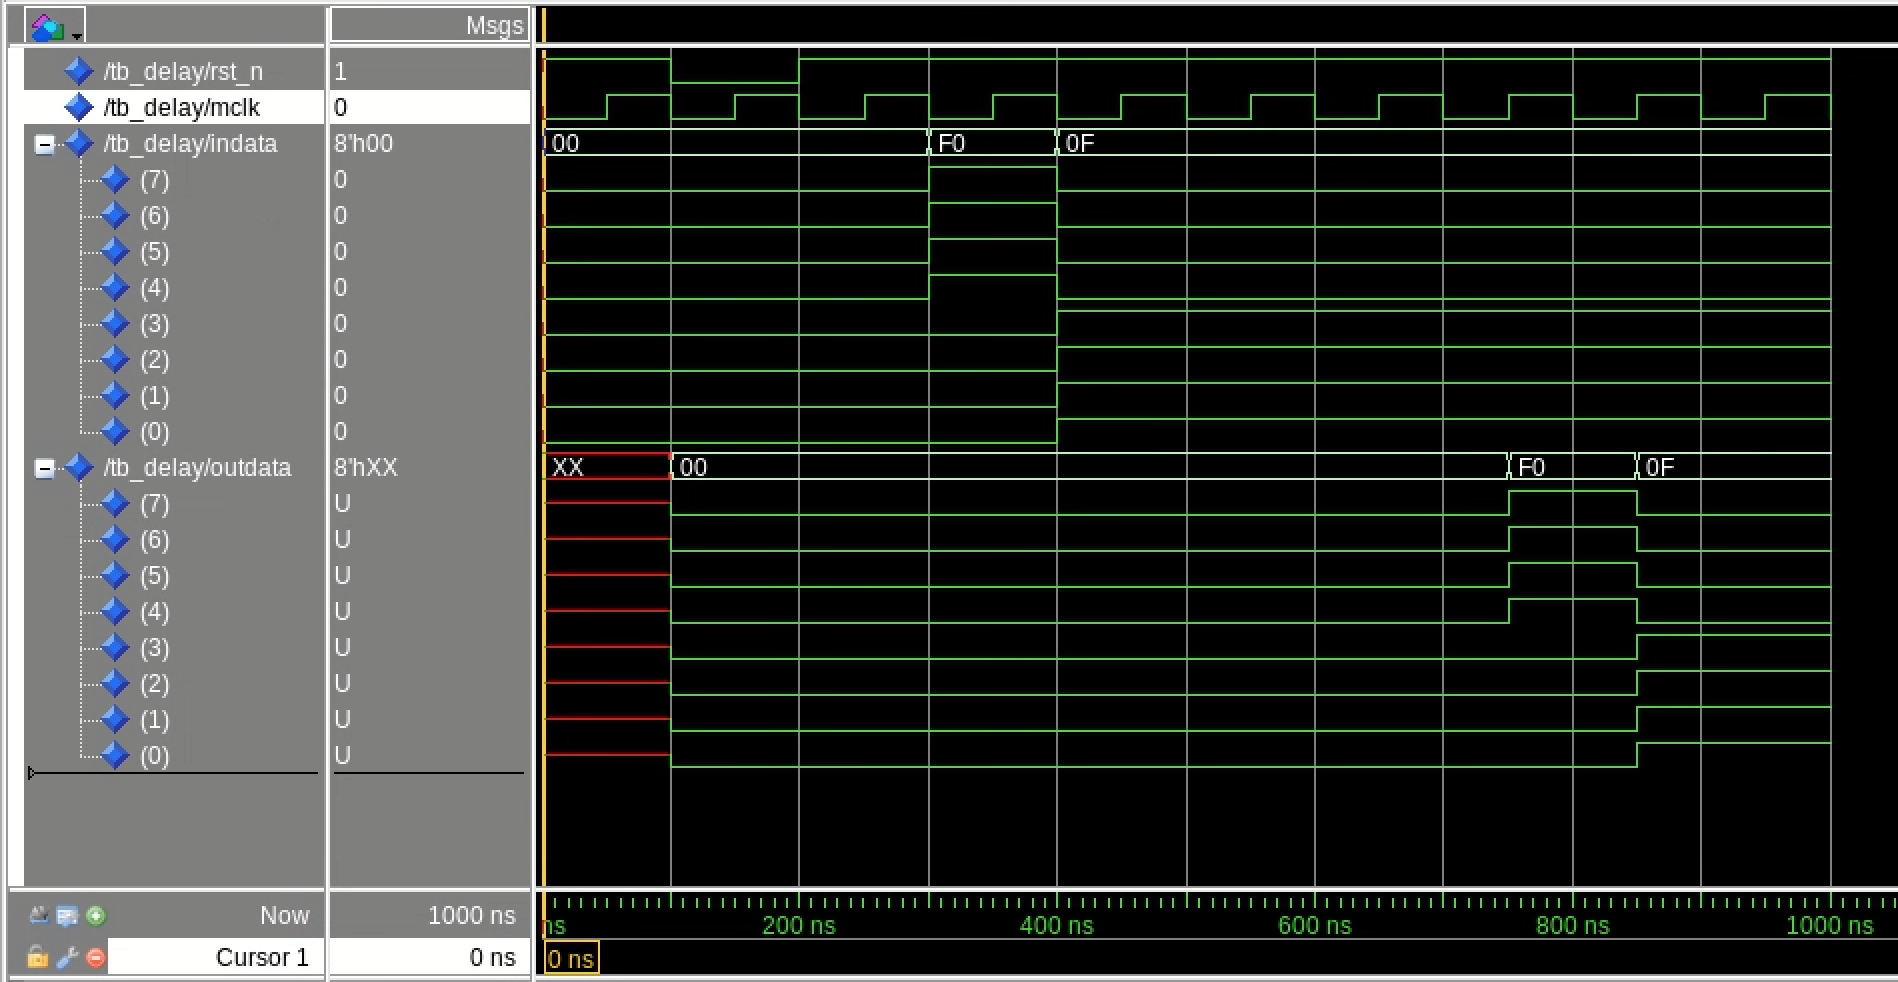
\includegraphics[width = \textwidth]{figur2.png}
            \caption{Task b}
            \label{fig:figure2}
        \end{figure} 
        \begin{figure}[!ht]
            \centering
            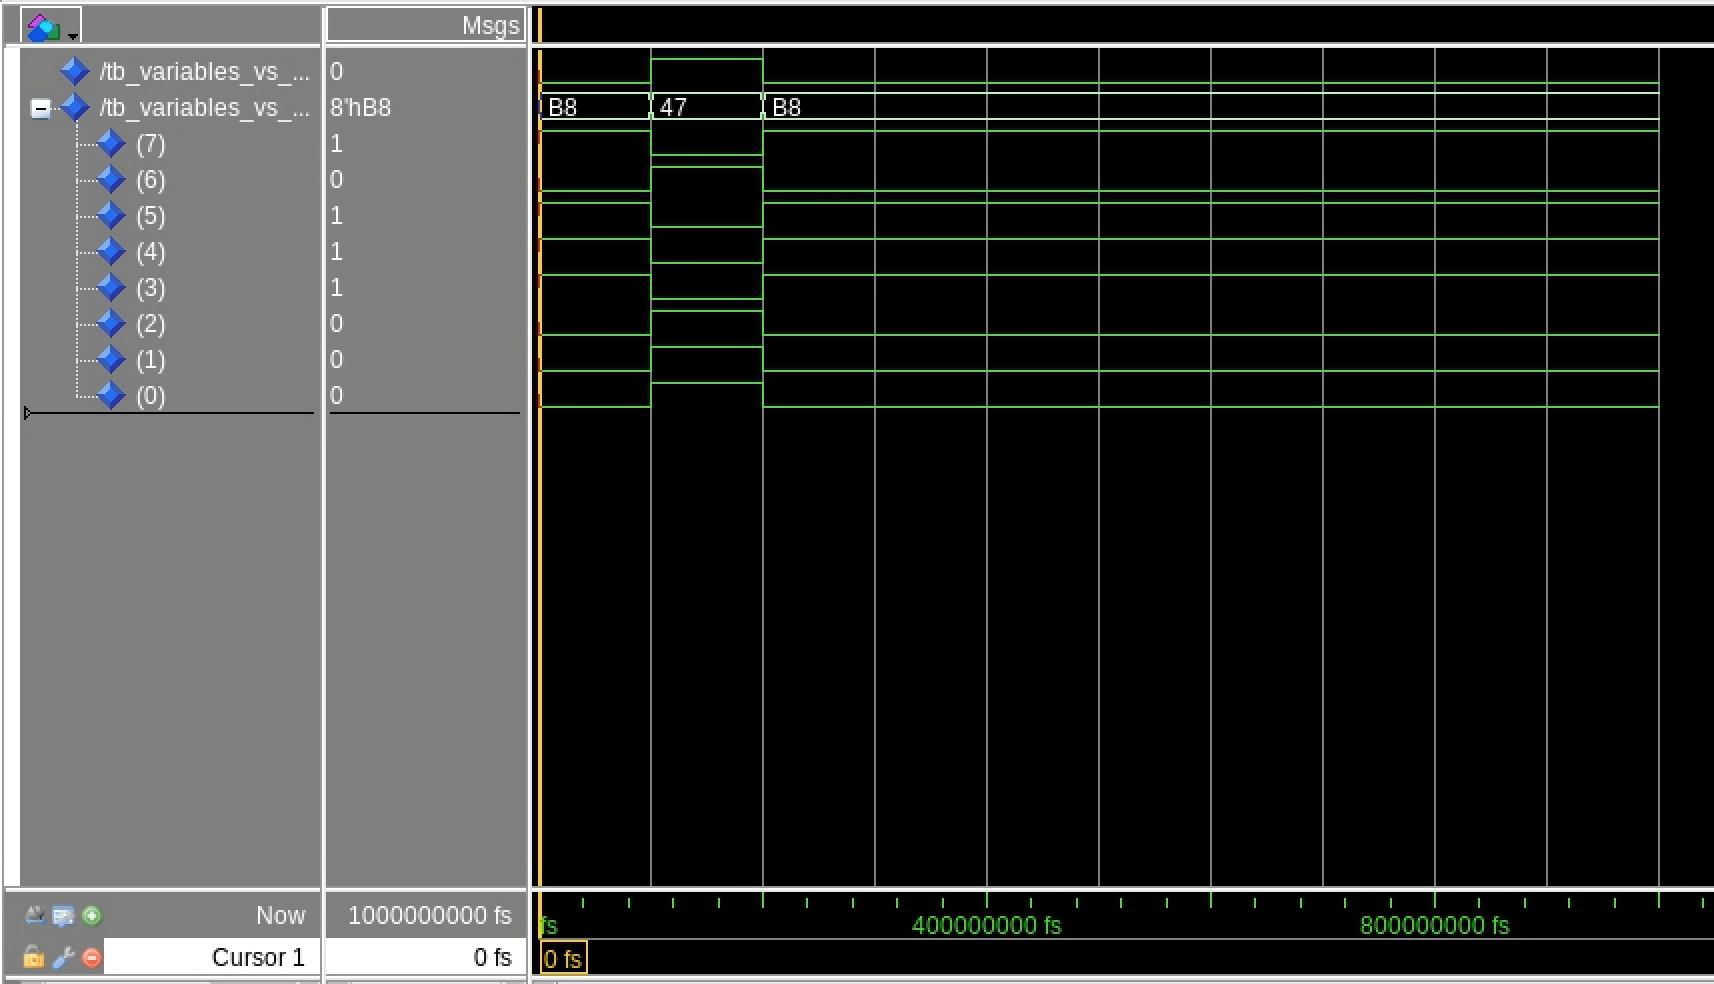
\includegraphics[width = \textwidth]{figur3.png}
            \caption{Task c}
            \label{fig:figure3}
        \end{figure}
        \begin{figure}[!ht]
            \centering
            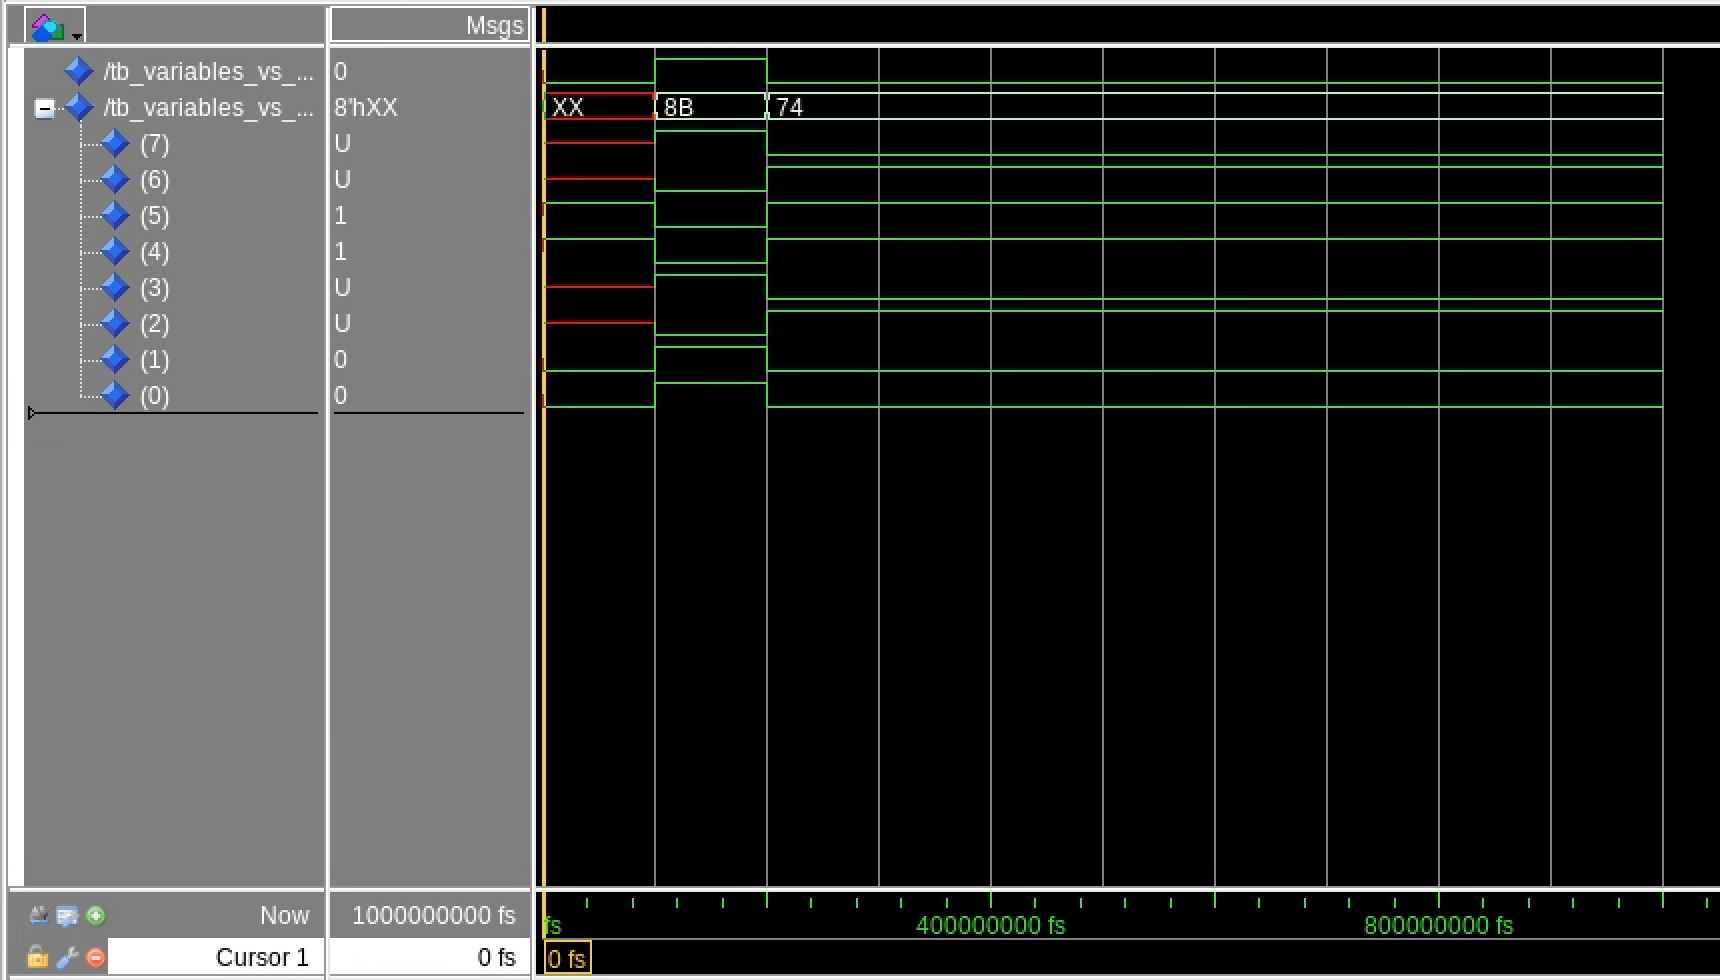
\includegraphics[width = \textwidth]{figur4.png}
            \caption{Task d}
            \label{fig:figure4}
        \end{figure}
\end{document}